\label{fs-formalism}

\subsection{Distributed streaming model}

\begin{definition}{Reference stream processing system}
\label{reference_system}
is a tuple of $(\Gamma,D)$, where $\Gamma$ is a set of all possible data flow elements, $D\subseteq{2^{\Gamma}\times2^{\Gamma}}$ is a binary relation on its power set. Computations within the system are defined by the recurrent rules on the set of input elements $A_\tau$, output elements $B_\tau$ and the reference working set $W^{*}_\tau$. On each iteration one of the following steps is chosen:

\begin{enumerate}
    \item \textbf{Input} $a_\tau\in{\Gamma}$:\\ $A_{\tau+1}=A_\tau \cup \{a_\tau\}, \\ B_{\tau+1}=B_{\tau}, \\ W^{*}_{\tau+1}=W^{*}_{\tau} \cup \{a_\tau\}.$
    \item \textbf{Output} $b_\tau\in{2^\Gamma}$:\\ $A_{\tau + 1} = A_{\tau}$, \\ $B_{\tau+1}=B_\tau \cup \{b_\tau\}, \\ W^{*}_{\tau+1}=W^{*}_{\tau} \setminus \{b_\tau\}.$
    \item \textbf{Transform}\\ $A_{\tau + 1} = A_{\tau}$,\\ $B_{\tau+1}=B_{\tau}$, \\ $W^{*}_{\tau+1}=(W^{*}_\tau \setminus X_\tau) \cup Y_\tau, (X_\tau,Y_\tau) \in D$, \\where\\$X_\tau \thicksim \mathcal{C}(\{X \subseteq W_\tau \cup B_\tau : \exists Y, (X,Y) \in D \}$, $\mathcal{C}$ is an unknown distribution). \label{random_formula}
\end{enumerate}

\end{definition}

Within our model, one can define a streaming system using only data flow elements and operations. Index $\tau\in{\mathbb{N}}$ can be considered as an exact global discrete time. We assume that only one event can happen at any single point in time $\tau$. We also suppose that output elements can be used in system transformations. This property is needed for snapshot and recovery mechanism introduced further. 

In a classical model proposed by Chandy and Lamport~\cite{Chandy:1985:DSD:214451.214456}, a distributed system is represented as a graph of processes, which can be connected to each other via channels. Each process can own a modifiable internal state, generate {\em events} and send them to other processes through the channels. {\em Global system state} in this model contains processes states and channel states, e.g., elements, which are in-flight at the moment. Distributed asynchronous processing is simulated using permutations of events.

The proposed model is a variation of a classical Chandy-Lamport distributed system model with the following properties and modifications:

\begin{itemize}
    \item Input and output elements $a_\tau$ and $b_\tau$ are special events. This way, {\em storage} and {\em computations} are distinguished. We assume that output elements $B_\tau$ are all data that leaves a system including so-called {\em state snapshots} which are typically used for recovery~\cite{Carbone:2017:SMA:3137765.3137777}. In most state-of-the-art stream processing systems, end-user is external to the system, i.e. a user is able to observe input and output elements, but not the working set.
    \item Our notion of a streaming system does not provide a concept of {\em operations state} because as it is shown in~\cite{we2018adbis}, states can be considered as ordinary data items. In this case, a state element is presented in a system until it is transformed into a new state together with new elements. This model allows a binary relation $D$ to capture computations within a graph of processes that is a physical streaming execution graph in our case. Hence, working set $W_\tau$ is a global state with only channel states in terms of Chandy-Lamport.
    \item Distributed asynchronous computations are modeled through the random choice of an operation that is executed next. Instead of using permutations of data flow elements which fixate an execution route, in the proposed model we suppose that the next transition of the working set is a random variable. For instance, this variable can be distributed uniformly or not according to the level of determinism. 
\end{itemize}

% We can imagine a working set as a pool, where some elements are poured in and others are poured out. Inside a pool, each element can be transformed into the other element, which can be transformed as well, and so on. Only survived elements are poured out from the pool. 

\begin{definition}{Probability of output element in a reference system}
$P(b_{\tau+1}|A_{\tau}, B_\tau)$ is a probability to observe output set $b$ at the time $\tau+1$ considering all previous input and output elements.
\end{definition}

For all output elements from the reference working set, such probability is positive, $\forall{b_{\tau+1} \in 2^{\Gamma}:\exists{W^{*}_{\tau+1}=W^{*}_{\tau}\setminus{b_{\tau+1}}}} \Rightarrow P(b_{\tau+1}|A_{\tau}, B_\tau) > 0$. It is important to note that there can be multiple reference working sets $\{W^{*}_{\tau+1}=W^{*}_{\tau}\setminus{b_{\tau+1}}\}$ due to asynchronous distributed processing. 

The reference stream processing system is just an abstract concept because it does not capture possible failures of network and computational units. Failure can be expressed as a loss of the working set or its part. There is a need to extend the reference model by a recovery mechanism that allows a system to transparently pass through the failures.

\begin{definition}{Stream processing system}
is a tuple of\\
$(\Gamma,D,F)$. Sets $\Gamma$ and $D$ define the reference system. Recovery function $F(A_\tau,B_\tau)$ provides logic for restoring of working set in case of system failures. Recurrent rules for computations are extended with a {\em recover transition}:
\begin{enumerate}
    \setcounter{enumi}{3}
    \item \textbf{Recover} \\  $A_{\tau + 1} = A_{\tau}$,\\ $B_{\tau+1}=B_{\tau}$, \\ $W_{\tau+1} = F(A_\tau,B_\tau)$
\end{enumerate}

\end{definition}

In this model, we suppose that {\em snapshots} of operation states taken by real stream processing systems are ordinary output elements. The motivation behind this assumption is the following:

\begin{itemize}
    \item Snapshots are typically stored in external systems, e.g. in HDFS, Kafka, relational databases, etc. They directly affect output elements after recovery.
    \item Stream processing systems aim at minimizing information which is needed to recover processing, but their optimizations do not directly affect consistency. The notion of $F(A_\tau,B_\tau)$ makes our concept general enough to describe any state-of-the-art streaming engine while being independent of a specific implementation of $F$.
\end{itemize}

\begin{definition}{Probability of output element in system with failures}
$P(b_{\tau+1}|A_{\tau}, B_\tau, F)$ is a probability to observe output element $b$ at the time $\tau+1$ considering all previous input and output elements, and recovery function.
\end{definition}

\subsection{Consistency guarantees}

The reference system concept allows us to express the notion of valid execution in terms of correspondence between input and output elements. In most real cases, input and output elements are the only data that can be observed by end-user. In real distributed stream processing systems, failures and recoveries can corrupt the output, despite the fact, that in terms of a naive definition of delivery guarantees, all elements are processed exactly once. Let us demonstrate it by an example. Assume that $\Gamma=\mathbb{N}$ and $D$ consists of a single non-commutative operation $V^{i+1}=a_\tau(1+V^{i}),V^{0}=0,V\in{S}$ and $\forall{t},b_t=V$. Upper index denotes an order of transformations. If $F(A_\tau,B_\tau)=F(A_\tau)$ system must set $V^{0}=0$ and reprocess input elements from the very beginning that seems like a naive but a correct approach for restoring. The system does not release output elements during reprocessing to preserve exactly once. However, if input elements arrive from asynchronous input channels, they can be reordered, and results of non-commutative operation may become inconsistent with results before the failure, e.g. the property of output monotonicity can be violated. This example is demonstrated in Figure~\ref{state-inconsistency}. 

\begin{figure}[htbp]
  \centering
  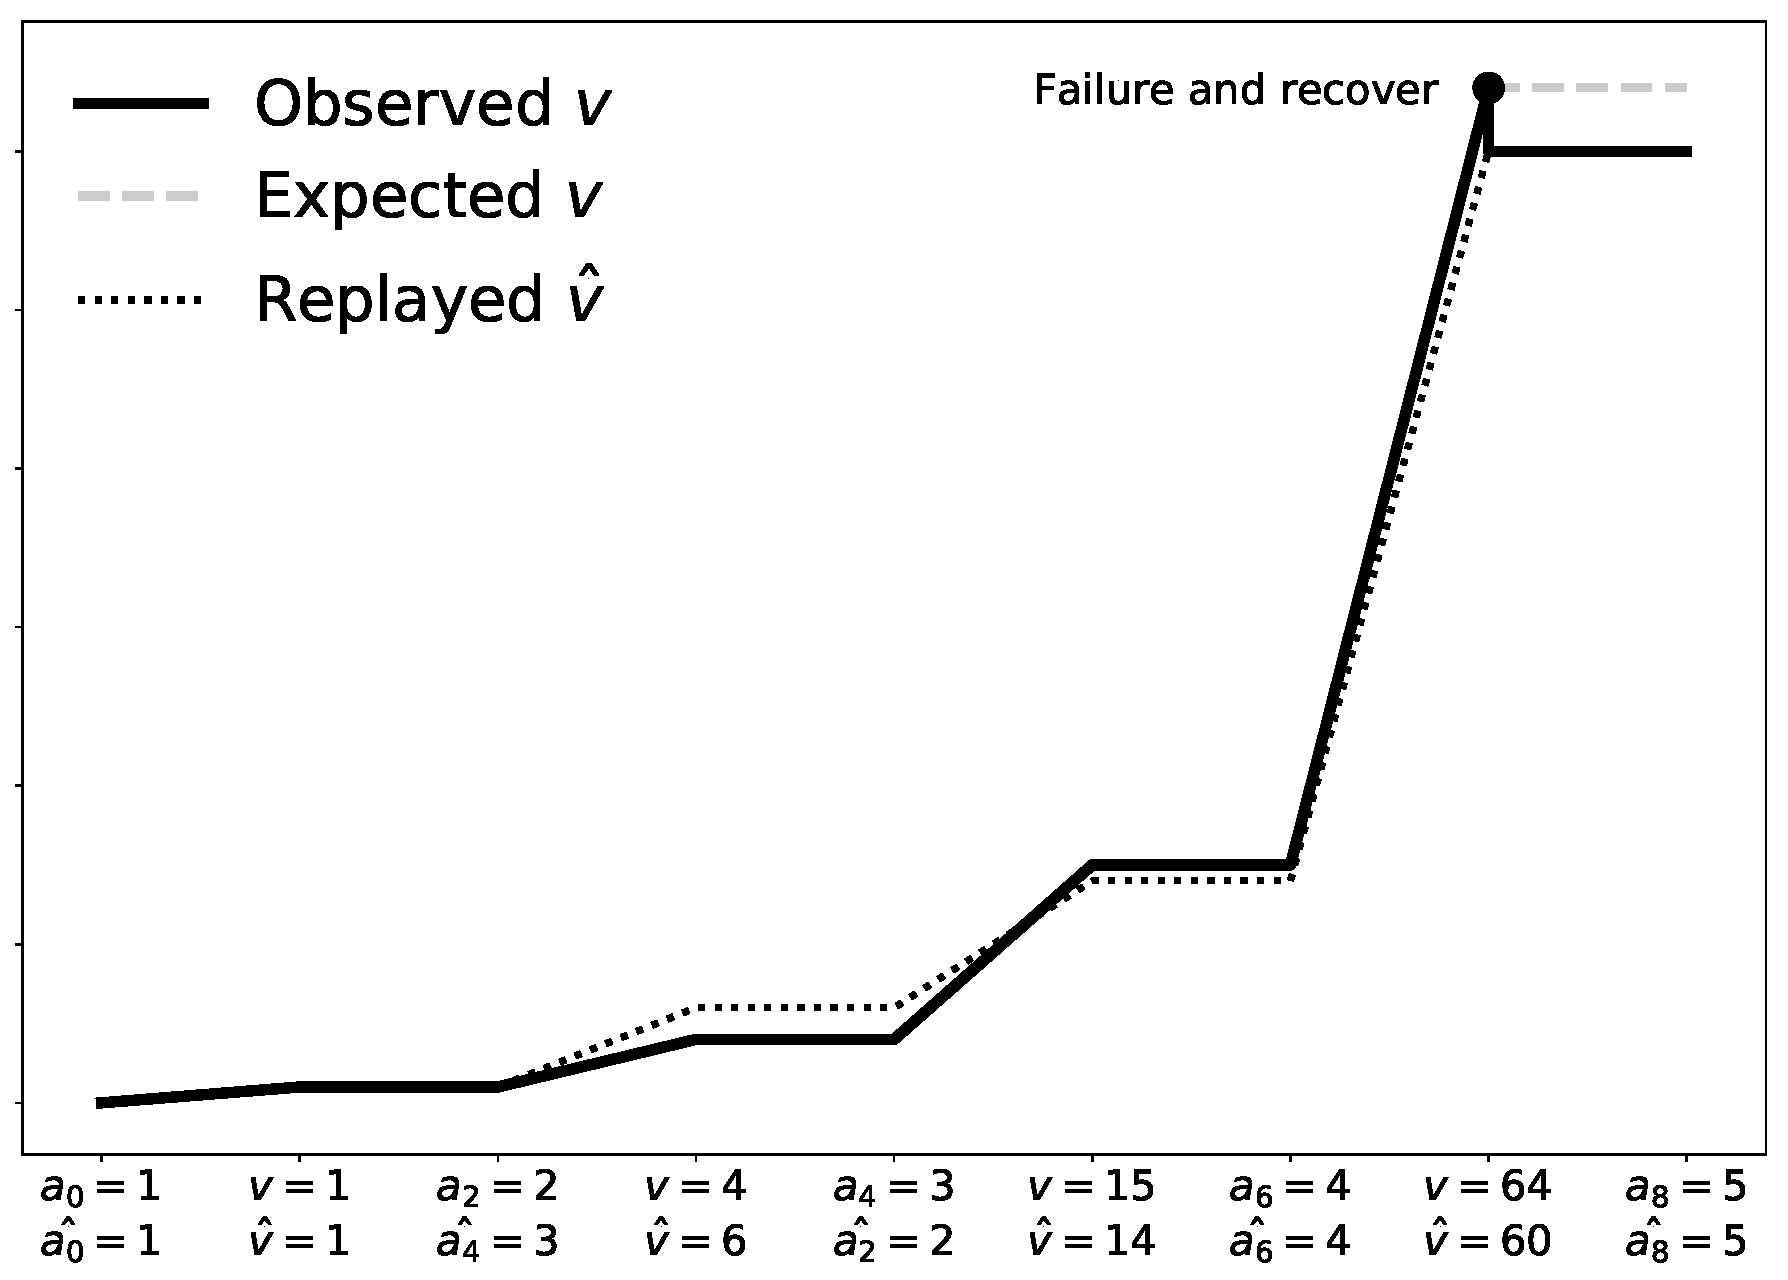
\includegraphics[width=0.48\textwidth]{pics/failure}
  \caption{Inconsistency of results after complete input reprocessing}
  \label {state-inconsistency}
\end{figure}

\begin{definition}{System provides for exactly once}
if it is possible to obtain each output element $b_{\tau+1}$ in the reference stream processing system, i.e.,\\ 
$\forall{\tau \in \mathbb{N}}, b_{\tau+1}\in 2^{\Gamma}: P(b_{\tau+1}|A_{\tau},B_\tau,,F)>0 \Rightarrow \\ P(b_{\tau+1}|A_{\tau},B_\tau)>0$.
\end{definition}

\begin{definition}{System provides for at most once}
if \\
$\exists{A^{0}_{\tau}\subseteq{A_{\tau}}}$ such that \\
$\forall{\tau \in \mathbb{N},{b_{\tau+1}\in 2^{\Gamma}}}: P(b_{\tau+1}|A_{\tau},B_\tau,F)>0 \Rightarrow \\ P(b_{\tau+1}|A^{0}_{\tau},B_\tau)>0$.
\end{definition}

\begin{definition}{System provides for at least once}
if \\
$\exists{A^{*}_{\tau}\subseteq{2^{A_{\tau}}}}$ such that \\
$\forall{\tau \in \mathbb{N}, {b_{\tau+1} \in 2^{\Gamma}}}: P(b_{\tau+1}|A_{\tau},B_\tau,F)>0 \Rightarrow \\ P(b_{\tau+1}|A^{*}_{\tau},B_\tau)>0$.
\end{definition}

Exactly once states that observed results cannot be distinguished from one of the possible results produced by the reference system. At most once and at least once guarantees are the relaxations of exactly once. The results within these guarantees can be obtained in the reference system, but with the assumption, that input is not completely correct. At least once can be reproduced if the input contains duplicated items. At most once can be achieved in the reference system if some input elements are missed. It is important to note, that regarding at most once guarantee we require an input element to be processed atomically with all its derivatives or not processed at all. To the best of our knowledge, no one real stream processing engine supports at most once guarantee, so we cannot verify the relevancy of this assumption. It is easy to provide at most once by producing no output at all but if the output is presented, at most once enforcement becomes much more difficult.  

In our formal model, the relaxations of exactly once are defined without diving into recovery mechanisms. Instead, they are described through possible input channel flaws in a reference system. This trick allows us to represent invisible system details in terms clear for a user.

Operations that are presented in $D$ can directly affect the complexity of consistency enforcement mechanisms. For example, if all operations are idempotent, exactly once can be obviously achieved~\cite{Akidau:2013:MFS:2536222.2536229}. On the other hand, if $D$ consists of non-idempotent and non-commutative, exactly once becomes challenging.

\begin{definition}{D contains non-commutative operation}
if\\ 
$\exists (x,y), s_1, s_2 \in \Gamma, s_1 \neq s_2: \\ ((x,y),s_1)\in D, \\ ((y,x),s_1)\notin D, \\ ((y,x),s_2)\in D$.
\end{definition}

\begin{definition}{System is deterministic}
if\\ 
$\forall{\tau\in{\mathbb{N}}, b_{\tau+1}\in{2^{\Gamma}}}:P(b_{\tau+1}|A_{\tau},B_\tau)=1$.
\end{definition}

An important property of a deterministic system is that it preserves the same order of elements before non-commutative operations on each run. The following theorem denotes the necessary and sufficient conditions for exactly once in non-deterministic systems with a non-commutative operation in $D$. It demonstrates that if a system is non-deterministic, but supports non-commutative operations, it must save (take a snapshot of) results of non-commutative operations before delivery of output elements that depend on these results.

\begin{theorem}
\label{necessary_conditions}
If $D$ contains non-commutative transformation, system supports exactly once if and only if $\forall F, a_\tau \in \Gamma, (x,y)\in Cl(D)(a_\tau), s\in Cl(x) \cap Cl(y), x\notin Cl(y), y\notin Cl(x), b_{\tau_1}, b_{\tau_2} \in Cl(s), \tau_2 > \tau_1 : b_{\tau_2} \in Cl(a_\tau) \setminus Cl^{-1}(D)(b_{\tau_1})$, where $s$ is obtained through non-commutative operation. The scheme of $D$ in the form of a graph is shown in Figure~\ref{???}. 
\end{theorem}
\begin{sketch}
$ $\newline
$\Rightarrow$

Assume that $b_{\tau_2} \notin Cl(a_\tau) \setminus Cl^{-1}(D)(b_{\tau_1})$ and system fails at time $\tau_1<\tau_f<\tau_2$. Let $\exists c \in Cl(s) \cap Cl^{-1}(D)(B_{\tau_2})$ and $c\neq b_{\tau_1}$. Then, to obtain $b_{\tau_2}$ there is a need to recompute $c$, and, therefore, $s$. However, due to asynchronous distributed processing and non-commutative transformation, system can reach not exactly $s$ such that $((x,y), s) \in D$, but $s':((y,x),s')\in D$. In this case, after recovery element $b_{\tau_2}$ will be delivered, but it will depend not on $s'$, but on $s$: $b_{\tau_2}\in Cl(D)(s')$. This is a contradiction, because $b_\tau$ has been already delivered and $P(b_{\tau_2}\in Cl(D)(s')|\{a_\tau\},\{b_{\tau_1} \in Cl(D)(s) \})=0$.

$ $\newline
$\Leftarrow$

Let system fails at time $\tau_f$. If $\tau_f < \tau_1$ or $\tau_f > \tau_2$, exactly once is obviously satisfied. Assume that $\tau_1<\tau_f<\tau_2$. In this case, $b_{\tau_1}\in B_{\tau_f}\subset B_{\tau_2}$. Hence, $b_{\tau_2}$ can be restored directly from $b_{\tau_1}$ without reprocessing of s, i.e. $F(a_\tau,b_{\tau_1})=b_{\tau_2}$ and $b_{\tau_1}, b_{\tau_2} \in Cl(s)$ after recovery.
\end{sketch}

In the proposed theorem, we assume that input element $a_\tau$ is split into elements $x,y$. The same behavior can be reproduced if two input elements $a_\tau$ and $a_{\tau+1}$ enter a system through asynchronous channels.

This theorem has a direct practical implication. If a system aims at providing exactly once, it must output elements only if there exists a snapshot that contains results of non-commutative operations. The problem here is that a system is usually not aware of user-defined operations and cannot distinguish commutative and non-commutative operations. It means that the lower bound of latency in the worst case in such systems is the snapshotting period together with the duration of taking a snapshot. There is a trade-off between latency and the frequency of taking snapshots because too frequent snapshotting can cause high extra load, while rare snapshots lead to high latency.

The property of determinism obviously allows a system not to satisfy the necessary condition from the Theorem~\ref{necessary_conditions}, because determinism guarantees order enforcement before non-commutative operations. Hence, if a system is deterministic, it is possible to inexpensively achieve a consistent snapshotting mechanism without synchronization between taking snapshots and output elements delivery. A deterministic system can release an element before a snapshot is taken. As we show further in experiments, this relaxation is able to dramatically decrease processing latency, because there is no need to wait until the snapshot is taken in order to release output elements.

To the best of our knowledge, only micro-batching systems support the property of determinism in streaming. However, micro-batching solutions provide higher latency than pure streaming engines due to overhead on input buffering~\cite{karimov2018benchmarking}. We proposed a pure streaming model called {\em drifting state}~\cite{we2018adbis} that allows achieving both determinism and low latency. Therefore, a question arises: is it more efficient in practice to handle non-determinism by atomic snapshotting and releasing than to maintain a fair determinism in order to get exactly once? 

It is important to note that the proposed model is suitable not only for the formal analysis of the properties of exactly once but for a deeper understanding of the other aspects of stream processing. While these topics are promising as well, they are out of the scope of this paper.

\subsection{Examples}

\subsubsection{MillWheel}

In MillWheel $\Gamma$ is all possible {\em records}. Dependency relation $D$ is set through a graph of user-defined transformations. In order to achieve exactly once, MillWheel atomically writes input and produced records of each operation to external storage. This behavior guarantees that results of all non-commutative operations are saved before delivery of its dependencies. Therefore, the conditions of the Theorem~\ref{necessary_conditions} are satisfied. Recovery function $F$ resends all saved records, but each operation deduplicates input records that have been already processed. The price for this exactly once enforcement technique is an overhead on external writes on each $\tau$~\cite{Akidau:2013:MFS:2536222.2536229}.    

\subsubsection{Flink}

In Flink, $\Gamma$ is represented as all {\em StreamRecords}. Relation $D$ is defined in the form of a directed acyclic graph consisted of user operations. Flink periodically saves information needed for recovery by injecting special elements called {\em checkpoints} into the input stream. Checkpoints go through the same network channels as ordinary elements and push all inverted dependencies of inputs through the system. Each operation prepares data to save independently at the moment of checkpoint arrival. Prepared data is committed to external storage when checkpoint passes through the whole data flow. Output elements are delivered to end-user only after the commit. This mechanism ensures that the results of non-commutative operations are saved before delivery of their dependencies that allows Flink to satisfy the Theorem~\ref{necessary_conditions}, but dramatically increases latency as we show further. Recovery function $F$ restores operation states and replays only input items which do not affect these states.

Besides overhead on snapshotting and delivery synchronization, checkpoints cause extra latency overhead because an operation with multiple inputs must wait until checkpoints arrive from each input. Only after that, an operation can safely send checkpoint further. This behavior is known as {\em checkpoints alignment}.

\subsubsection{Spark streaming}

In Spark Streaming, $\Gamma$ is a set of all possible {\em RDDs}. Unlike pure streaming engines like Flink and MillWheel, where input elements arrive one by one, RDD is a small collection of data that is atomically processed. Dependency relation on the power set of $\Gamma$ is also defined using a directed acyclic graph of user operations. Spark inherits main properties form batch processing systems including the fact that each new stage of computations is started only after the previous one is completed. This fact ensures fulfillment of the Theorem~\ref{necessary_conditions} and makes it simple to achieve determinism. Recovery function $F$ restores just the last non-complete stage.
 
To the best of our knowledge, spark streaming is the only state-of-the-art stream processing system that provides for deterministic results. However, an architecture based on the processing of collections of buffered input elements ({\em micro-bathing}) makes it hard to achieve latency lower than several seconds~\cite{7530084, 7474816}. 
